
%%%%%%%%%%%%%%%%%%%%%%%%%%%%%%%%%%%%%%%%%%%%%%%%%%%%%%%%%%%%%%%%%%%%%%%%%%%%%%
% Copyright (c) 2003-2014 by University of Queensland
% http://www.uq.edu.au
%
% Primary Business: Queensland, Australia
% Licensed under the Open Software License version 3.0
% http://www.opensource.org/licenses/osl-3.0.php
%
% Development until 2012 by Earth Systems Science Computational Center (ESSCC)
% Development 2012-2013 by School of Earth Sciences
% Development from 2014 by Centre for Geoscience Computing (GeoComp)
%
%%%%%%%%%%%%%%%%%%%%%%%%%%%%%%%%%%%%%%%%%%%%%%%%%%%%%%%%%%%%%%%%%%%%%%%%%%%%%%

\chapter{The \ripley Module}\label{chap:ripley}
%\declaremodule{extension}{ripley}
%\modulesynopsis{Solving linear, steady partial differential equations using finite elements}

\ripley is a specialised form of \finley, supporting structured, 
uniform meshes with rectangular elements in 2D and hexahedral elements 3D.
Uniform meshes allow a straightforward division of elements among processes
with \MPI and allow for a number of optimizations when solving PDEs.
\ripley also supports fast assemblers for certain types of PDE (specifically
Lam\'e and Wave PDEs).
These assemblers make use of the regular nature of the domain to optimize the
stiffness matrix assembly process for these specific problems.
Finally, \ripley is currently the only domain family that supports GPU-based
solvers.

As a result, \ripley domains cannot be created by reading from a mesh file
since only one element type is supported and all elements need to be equally
sized.
For the same reasons, \ripley does not allow assigning coordinates via
\function{setX}.
Other than that \ripley and \finley are generally interchangeable in a script
with both modules having the \class{Rectangle} or \class{Brick} functions
available. Consider the following example which creates a 2D \ripley domain:

\begin{python}
 from esys.ripley import Rectangle, Brick
 dom = Rectangle(9, 9)
\end{python}

\section{Formulation}
For a single PDE that has a solution with a single component the linear PDE is
defined in the following form:
\begin{equation}\label{eq:ripleysingle}
\begin{array}{cl} &
\displaystyle{
\int_{\Omega}
A_{jl} \cdot v_{,j}u_{,l}+ B_{j} \cdot v_{,j} u+ C_{l} \cdot v u_{,l}+D \cdot vu \; d\Omega }
+ \displaystyle{\int_{\Gamma} d \cdot vu \; d{\Gamma} }\\
= & \displaystyle{\int_{\Omega}  X_{j} \cdot v_{,j}+ Y \cdot v \; d\Omega }
+ \displaystyle{\int_{\Gamma} y \cdot v \; d{\Gamma}}
\end{array}
\end{equation}

\section{Meshes}
\label{sec:ripleymeshes}
An example 2D mesh from \ripley is shown in Figure~\ref{fig:ripleyrect}.
Mesh files cannot be used to generate \ripley domains, i.e. \ripley does not
have \function{ReadGmsh} or \function{ReadMesh} functions.
Instead, \ripley domains are always created using a call to \function{Brick}
or \function{Rectangle}, see Section~\ref{sec:ripleyfuncs}.

\begin{figure}
\centerline{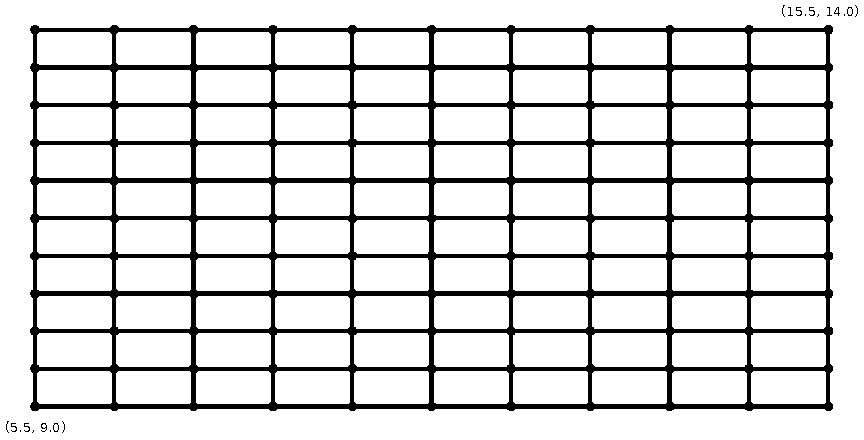
\includegraphics{RipleyMesh}}
\caption{10x10 \ripley Rectangle created with \var{l0=(5.5, 15.5)} and
\var{l1=(9.0, 14.0)}}
\label{fig:ripleyrect}
\end{figure}

\section{Functions}\label{sec:ripleyfuncs}
\begin{funcdesc}{Brick}{n0,n1,n2,l0=1.,l1=1.,l2=1.,d0=-1,d1=-1,d2=-1,
diracPoints=list(), diracTags=list()}
generates a \Domain object representing a three-dimensional brick between
$(0,0,0)$ and $(l0,l1,l2)$ with orthogonal faces. All elements will be regular.
The brick is filled with
\var{n0} elements along the $x_0$-axis,
\var{n1} elements along the $x_1$-axis and
\var{n2} elements along the $x_2$-axis.
If built with \MPI support, the domain will be subdivided 
\var{d0} times along the $x_0$-axis,
\var{d1} times along the $x_1$-axis, and
\var{d2} times along the $x_2$-axis.
\var{d0}, \var{d1}, and \var{d2} must be factors of the number of
\MPI processes requested.
If axial subdivisions are not specified, automatic domain subdivision will take
place. This may not be the most efficient construction and will likely result in
extra elements being added to ensure proper distribution of work. Any extra
elements added in this way will change the length of the domain proportionately.
\var{diracPoints} is a list of coordinate-tuples of points within the mesh,
each point tagged with the respective string within \var{diracTags}.
\end{funcdesc}

\begin{funcdesc}{Rectangle}{n0,n1,l0=1.,l1=1.,d0=-1,d1=-1,
diracPoints=list(), diracTags=list()}
generates a \Domain object representing a two-dimensional rectangle between
$(0,0)$ and $(l0,l1)$ with orthogonal faces. All elements will be regular.
The rectangle is filled with
\var{n0} elements along the $x_0$-axis and
\var{n1} elements along the $x_1$-axis.
If built with \MPI support, the domain will be subdivided 
\var{d0} times along the $x_0$-axis and
\var{d1} times along the $x_1$-axis.
\var{d0} and \var{d1} must be factors of the number of \MPI processes requested.
If axial subdivisions are not specified, automatic domain subdivision will take
place. This may not be the most efficient construction and will likely result in
extra elements being added to ensure proper distribution of work. Any extra
elements added in this way will change the length of the domain proportionately.
\var{diracPoints} is a list of coordinate-tuples of points within the mesh,
each point tagged with the respective string within \var{diracTags}.
\end{funcdesc}

\noindent The arguments \var{l0}, \var{l1} and \var{l2} for \function{Brick}
and \function{Rectangle} may also be given as tuples \var{(x0,x1)} in which
case the coordinates will range between \var{x0} and \var{x1}. For example:
\begin{python}
   from esys.ripley import Rectangle
   dom = Rectangle(10, 10, l0=(5.5, 15.5), l1=(9.0, 14.0))
\end{python}

\noindent This will create a rectangle with $10$ by $10$ elements where the
bottom-left node is located at $(5.5, 9.0)$ and the top-right node has
coordinates $(15.5, 14.0)$, see Figure~\ref{fig:ripleyrect}.

\section{Linear Solvers in \SolverOptions}
Currently direct solvers and GPU-based solvers are not supported under \MPI
when running with more than one rank.
By default, \ripley uses the iterative solvers \PCG for symmetric and \BiCGStab
for non-symmetric problems.
A GPU will not be used unless explicitly requested via the
\function{setSolverTarget} method of the solver options.
These solvers are only available if \ripley was built with \CUDA support.
If the direct solver is selected, which can be useful when solving very
ill-posed equations, \ripley uses the \MKL\footnote{If the stiffness matrix is
non-regular \MKL may return without a proper error code. If you observe
suspicious solutions when using \MKL, this may be caused by a non-invertible
operator.} solver package. If \MKL is not available \UMFPACK is used.
If \UMFPACK is not available a suitable iterative solver from \PASO is used.



